\documentclass[12pt]{paper}
\usepackage{amsmath}
\usepackage{amssymb}
\usepackage{graphicx}
\usepackage{hyperref}
\usepackage{color}
\begin{document}
\title{Definitions-Biology}
\maketitle
\section{Histones}
...

Hyperaccetlation of the histones leads to unfolding of the chromatin that should facilitate the general accessibility of factors to the DNA \cite{Blackwood98}.

\section{Enhancers}
 An \href{http://en.wikipedia.org/wiki/Enhancer_(genetics)}{Enhancer} is a short (20-400bp,\cite{Kulaeva12}) region of DNA that can be bound with proteins to activate transcription of a gene or genes. These proteins are usually referred to as transcription factors. Enhancers contain  specific sequence motifs with which DNA-binding proteins interact and transmit molecular signals to genes \cite{Blackwood98}.

Enhancers increase transcription of genes in a manner that is independent of their orientation and distance relative to the RNA start site \cite{Blackwood98} 


\section{Promoters}
Promoters (or core promoters) are located within $\pm 40$ nucleotides from the RNA start site \cite{Blackwood98}. Promoters are identified according to their TATA box. 


\section{TATA box}
Considered to be the core promoter region, it is a short sequence of DNA and, which acts as the binding site for general transcription factors. TATA box contains the sequence 5'-TATAAA-3' . It is usually located within 25 bp of the transcription start site. About 24$\%$ of the genome contains TATA box sites. In the process of transcription, the TATA binding protein binds to the TATA box an unwinds the DNA. Because the TATA box is rich with AT connections, it facilitates easier unwinding of the DNA, due to the weaker base-pair interactions). Most genes lack TATA box and use instead an initiator element. Only about 10$\%$ of the promoters in humans depend on TATA boxes. 

\section{Insulators}

\section{Promoter-Enhancer Interactions}
In the majority of cases, action of enhancers involves enhancer-promoter interaction through proteins bound at the enhancer and promoter, accompanied by formation of an intervening chromatin loop \cite{Kulaeva12}.

There are two mechanisms by which enhancer-promoter  selectivity might be achieved. First, there could be specific interactions between enhancer -binding proteins and factors that interact with the promoter. Second, boundary elements (insulators) could be used to block undesired enhancer-promoter interactions \cite{Blackwood98}. 

How might enhancer binding proteins and their associated co-activators  establish productive interaction with the promoter? One option is the DNA looping. A "facilitated tracking" mechanism for enhancer function is postulated to allow enhancer bound complex containing DNA-binding factors and co-activators "tracks" via small steps along the chromatin until it encounters the promoter, at which a stable looped structure is formed \cite{Blackwood98}. After formation of the activation chromatin loop, it is likely stabilized by additional protein factors, such as CTCF and cohesin \cite{Kulaeva12}. CTCF is an insulator DNA binding protein. 


It was shown that formation of chromatin loop topologically isolating the enhancer from the target promoter is sufficient to block enhancer-promoter communication. 


For an illustration of the participants in gene transcription see Figure \ref{mechanismOfGeneTranscription}

\begin{figure}[H]
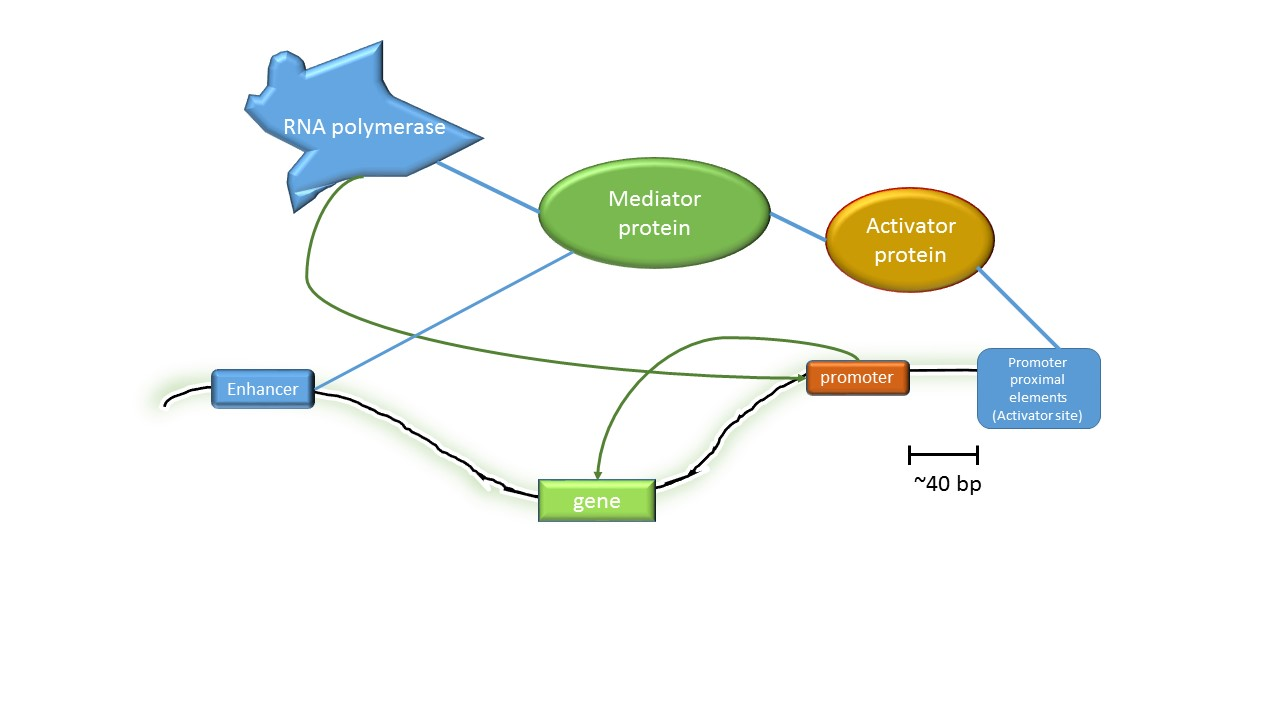
\includegraphics[scale=0.5]{mechanismOfGeneTransciption}
\caption{The participants in the process of gene transcription. The enhancer is connected to the mediator protein which recruits RNA polymerase to the process. The mediator gene is connected to the activator protein, which is connected to promoter proximal elements. These elements are located within $\sim$40 bp of the promoter, a property which allows the RNA polymerase to quickly find the promoter and to initiate transcription}
\label{mechanismOfGeneTranscription}
\end{figure}

% The bibliography
\bibliographystyle{plain}
\bibliography{thebibliography} % the bibliography.bib file 
\end{document}